%必要事項
%論文に目を通す
%"音楽の表現"の修正
%追加すべき事項
% - "音楽の表現"の式(理解が必要)
% - "音楽の表現"の具体例(論文,既存研究)
% - "音楽の表現"の図
% - "音楽の表現"の単語の説明
\chapter{背景:音楽}

本章では、本論文での音の定義を行った後に、音楽の特徴量抽出の方法を紹介する。

\section{音の定義}

音とは、弾性体中を伝播する弾性波により起こされる音波が聴覚により感じられるもののことである。また、音は騒音と楽音の大きく二つに分けることができる。騒音とは不規則な振動の音波による音のことであり、楽音とは周期性のある音波による音のことである。そして、本論文では楽音を音と定義するが、楽音は長さ、大きさ、高さ、音色の四要素を持つ。ここで、\prettyref{fig:gakuon1}はある音波の図であり、\prettyref{fig:gakuon2}はその音波の適当な部分の拡大図である。

\subsection{音の長さ}

音の長さは音波の時間長として定義する~(\prettyref{fig:gakuon1})~。また、音の長さは楽譜上での時間の長さ~(音価)~として一般には定義される。

\subsection{音の大きさ}

音の大きさは音波の振幅により決まる~(\prettyref{fig:gakuon1})~。また、人間は振幅の大きい音ほど大きく知覚する。

\begin{figure}[b]
\centering
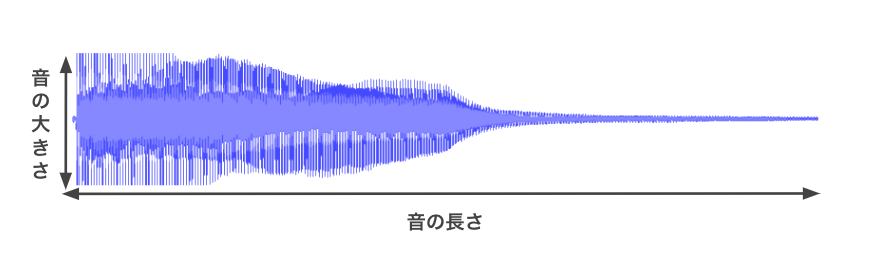
\includegraphics[width=\hsize]{figure/gakuon1.png}
\caption{音波}
\label{fig:gakuon1}
\end{figure}

%ここで改ページ

\subsection{音の高さ}

音の高さは音波の周波数により決まる。直感的には、音波の周期構造の長さにより決まる~(\prettyref{fig:gakuon2})~。また、人間は周波数の高い音ほど高く知覚する。

\subsubsection{単音と重音}

ある楽器である高さの一音を鳴らした時に出力される音を単音と呼ぶ。また、ほとんどの単音は複数の周波数の音波の合成波であり、最も低い周波数成分の音~(基音)~の高さを音の高さとして人間は知覚する。そして、この単音の音を重ね合わせた音のことを重音と呼ぶ。

\subsubsection{音階表記}

本論文では、西洋音楽で用いられる12音階の表記を音の高さを表すために使用する。この表記では、$C,C^{\sharp},D,D^{\sharp},E,F,F^{\sharp},G,G^{\sharp},A,A^{\sharp},B$の12段階の音の高さの集合をオクターブとして定める。そして、それぞれのオクターブに番号を振り、440~Hzの音をA4と定めることで音の高さの絶対的な表記を可能にしている。また、この表記で表す音を半音と呼ぶが、半音より細かい音~(微分音)~を表すことはできない。ただし、本論文では半音のみを音の高さとして扱う。

\subsection{音の音色}

音の長さと大きさと高さが同じであっても異なった音として人間には知覚されることがある。この違いを音色と呼び、別の楽器は異なった音色を持つ。直感的には、音色は音波の周期構造の形により決まる~(\prettyref{fig:gakuon2})~。また、この周期構造の違いは基音より高い音~(上音)~の音波の組み合わせの違いに起因する。

\begin{figure}[b]
\centering
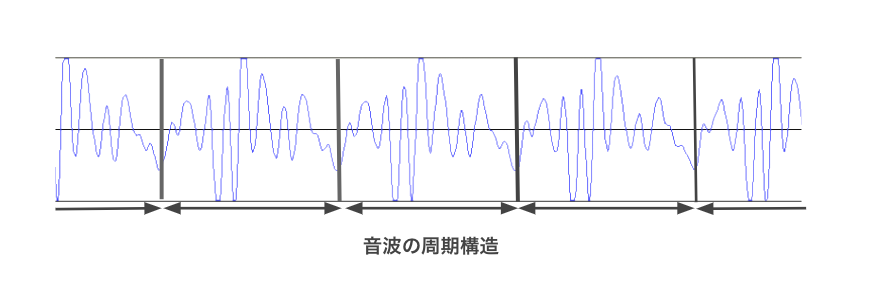
\includegraphics[width=\hsize]{figure/gakuon2.png}
\caption{音波の拡大図}
\label{fig:gakuon2}
\end{figure}

%ここで改ページ(したい)

\section{音楽の特徴}

一般には音楽で特定の音色への変換を行うことは難しいが、本研究では三つの要素に分解することで単音での音色の変換を音楽へと適用することが可能であると考えた。

\subsection{楽器の重ね合わせ}
    
音楽はそれぞれの楽器から出力される音の重ね合わせになっている。楽器ごとに音色は異なるため、音色変換を行うには楽器ごとの音波に分解すること~(音源分離)~が必要であると考えられる。なお、楽曲の作成時に楽器ごとに分離したデータ~(パラデータ)~として保存することが一般的であるため、パラデータの公開が一般的になれば音源分離の必要はなくなる。

\subsection{音の重ね合わせ}

ある音が重音である場合はそれぞれの単音について音色変換を行う必要がある。本研究では、データセットとして単音のみを使用するが、重音もデータセットに加えることで音色変換が可能であると考えられる。また、この際にデータセットが膨大な量になる可能性があり、追加するデータセットの工夫が必要である。

\subsection{音の繋ぎ方}

楽器ごとの音波に分解可能で重音も表現可能である時、時間方向の音の繋ぎ方を工夫する必要がある。また、単音の変換を一定の単位時間で行うことで、音楽もその単位時間で分割して変換することで可能であると考えられる。ただし、単位時間の定め方により性能が変わると考えられるので、単位時間は慎重に定める必要がある。

%ここで改ページ

\section{音楽の表現}
\label{sec:preprocess}

ニューラルネットワークで音楽を扱うためには表現の工夫が必要である。以降の内容は~\cite{musictutorial}を参考に作成した。

\subsection{一次元データと二次元データ}

まず、基本的な表現は一次元データの音響信号であるが、ほとんどの場合は何らかの加工を施した二次元データである。また、二次元の軸としては周波数と時間を選ぶことが多い。この時、音楽のどのような特徴を把握したいか及びネットワークの時間計算量と空間計算量に合わせて適切な表現を選ぶ必要がある。

そして、多くの場合、二次元データでは中心周波数を利用したフィルタを用いて音響信号を分解し、信号を明確化する。これにより、効果的なデータ表現として扱うことができる。さらに、二次元の場合は画像と同じアルゴリズムを用いることができるが、異なる特徴が存在する。まず、画像の場合は局所的な相互関係が存在する。例えば、近くのピクセル同士は色合いや強度が似ている。しかし、スペクトログラムでは、周波数成分の方向で調和的な関係は存在する一方で局所的な相互関係は弱い。また、調和的な関係を把握するために表現を変更するような研究もある。そして、物体認識ではスケール不変性も求められるが、音楽についてはあまり関係はないと考えられる。

\subsection{音響信号}

音響信号とは信号としての音の呼び名である。また、連続量である音響信号~(アナログ信号)~はコンピュータではデジタル信号に変換されて処理される。この時、標本化~(サンプリング)~と量子化が必要である。サンプリングとはアナログ信号を一定の間隔を空けて離散的に測定を行うことであり、量子化とは信号の大きさを離散的に近似して表現することである。そして、1秒あたりのサンプリング回数をサンプリング周波数、信号の大きさを表現するビット数を量子化ビット数、と呼ぶ。

音響信号は一次元の音の素朴な表現であるが、ニューラルネットワークの学習により音の特徴を把握するには多くのデータセットが必要になると考えられ、以降で紹介する二次元での表現へと変換されて扱われることが多い。ただ、〇〇などの研究では音響信号のままニューラルネットワークを用いることがあり、本研究ではこちらの音響信号の形で音を扱った。

\subsection{STFT}

STFTは線形間隔の中心周波数を用いて周波数成分を分解し、時間-周波数の二次元の表現を行う方法である。また、高速フーリエ変換を用いることにより、他の二次元の表現と比べて高速に計算を行うことができる。

しかし、線形間隔の中心周波数の利用は音楽に適しているとは言えない。なぜなら、人間の知覚系の周波数分解能は線形とかなり異なるからである。また、STFTは音楽の解析のために作られたわけでもないからである。これらの理由から、STFTはディープラーニングにおいては最も人気のある手法ではない。

ただし、STFTの音響信号との間の可逆性を利用して、音源分離などに用いられる。

\subsection{メルスペクトログラム}

メルスペクトログラムは人間の知覚系に合わせて最適化された二次元の表現であ李、STFTにおいて周波数方向に関してメル尺度~\cite{melscale}を用いて圧縮を行ったものである。そのため、知覚として必要な情報を保持したまま圧縮を行うことができる。ただし、メルスペクトログラムは位相の情報を保持せず音の大きさのみを保持しているため、音響信号との間で非可逆的である。

また、メル尺度を表す式にはいくつかあり、\prettyref{eq:mel}はその一つである。

\begin{align}
    \label{eq:mel}
\end{align}

経験的かつ心理的な理由でメル尺度を用いたメルスペクトログラムは音楽のタスクに適している。(例もある)

\subsection{CQT}

CQTは対数振幅の中心周波数を使用した二次元の表現である。CQTは対数振幅を用いており、音の高さの分布に近い。したがって、基音を正確に識別する際に用いられ、和音の識別や書き換えに使うことができる。

また、計算量としてはSTFTやメルスペクトログラムより重い。そして、単純な対数振幅のスペクトログラムが有効な例もある。

\subsection{クロマグラム}

与えられた音の高さの集合におけるエネルギー分布のこと。多くの場合は西洋音楽の12音階をその集合とする。つまり、クロマグラムは周波数方向に畳み込んだCQTと見なすことができる。また、クロマグラムは他の表現方法よりも処理が進んだものなので、それ自身を特徴量として用いることができる。